Based on the discussed practical applications and novel visualization approaches, one can see that there is no such tool combining thematic maps with animations when changing visual appearance. The advantages and disadvantages of all aspects have been broached and discussed. This thesis will furthermore discuss and show a novel approach based on the concept of unit visualizations combined with classical thematic maps and animations when changing visual appearance. However, there are multiple possible solutions. This section will discuss some solutions with the requirement of building an an interactive web application. The solutions should yield answers to the question of which tasks can be supported by particle aggregation in thematic maps and how can the aggregation be realized.

In order to realize a practical solution for the given question, it is assumed that a dataset including heterogeneous data and some kind of geospatial data is given.

According to the mantra of \citeauthor{Shneiderman1996}, the application should start by giving an overview of the dataset. With the main concept in mind, there are two possible solutions:
\begin{enumerate}

\ditem{Unit-based grid} \hfill \\
SandDance features an approach of showing a grid as visualization, where all data items are represented as some kind of shape. Figure \ref{fig:sanddance-grid} on page \pageref{fig:sanddance-grid} shows the implementation of a unit-based grid.

\begin{figure}[!htb]
\centering
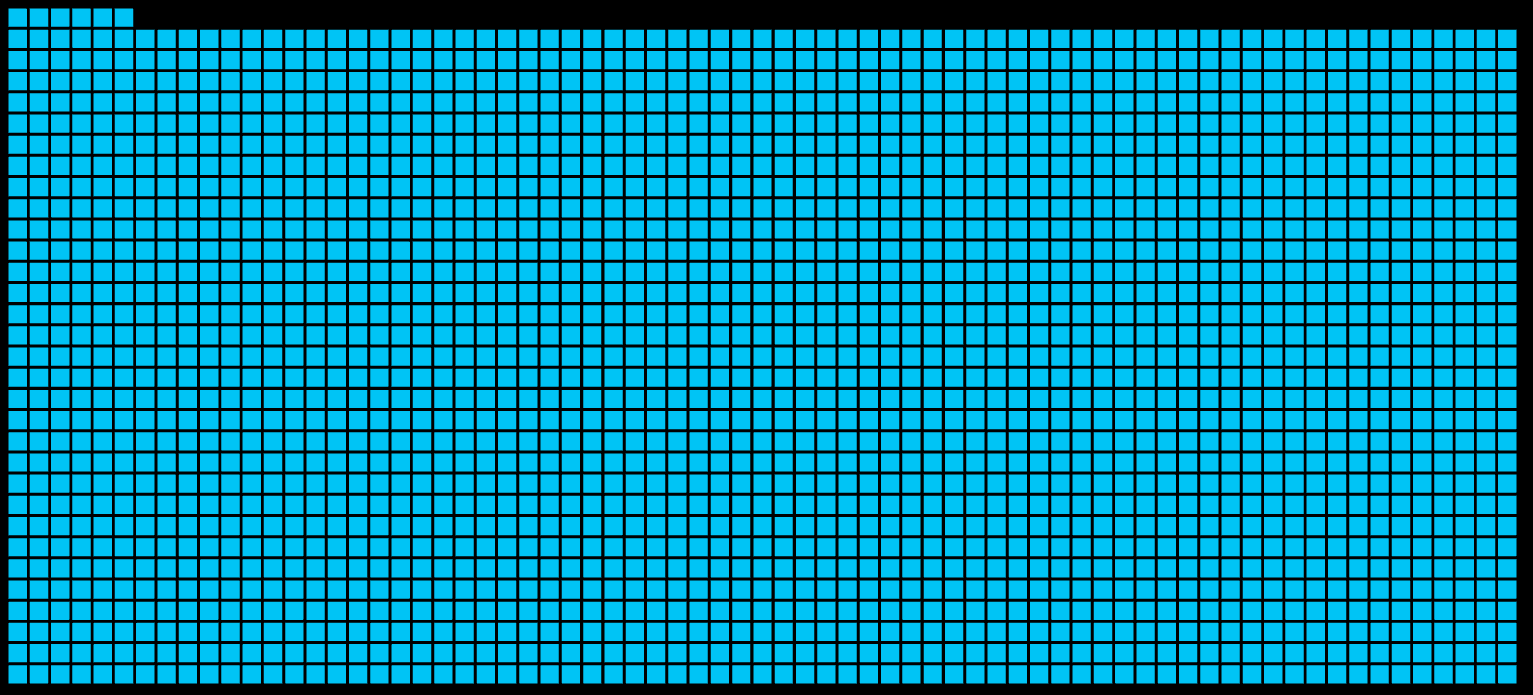
\includegraphics[height=5cm]{images/methods/related/sanddance-grid.png}
\caption[
    Unit-based grid in SandDance.
]{Unit-based grid in SandDance}
\label{fig:sanddance-grid}
\end{figure}

\ditem{Dot map} \hfill \\
Chapter \ref{s:dot} on page \pageref{s:dot} discusses the concept of dot maps in detail. This kind of thematic map can be used in combination with a one-to-one relation ship and show every item in the dataset as a single dot on the map giving an overview of the whole dataset including its geographical distribution.
\end{enumerate}

The next step after having an overview is to decide which tasks to try out in order to test particle aggregation. One big part of this thesis already dicsusses thematic cartography in detail and thus the decision of using different types of thematic maps, which are all based on some kind of aggregation, is reasonable. Therefore trying animated particle aggregation in combination with proportional symbol maps, choropleth maps and cartograms will be a main part of the practical approach. However, there are multiple ways in changing visual appearance from an overview of the data to some kind of thematic map.

\begin{enumerate}

\ditem{In-place transition} \hfill \\
Changing from one kind of a thematic map to another one with in-place transition denotes the concept of creating the upcoming visualization. Starting with an overview grid and having a dot map as an upcoming visualization would move all particles in the same canvas to their geographical position. Having a map in the background when changing from an abstract grid to a thematic map could support the comprehensibility.
If the user determines to change the visual appearance to some other kind of thematic map, the particles would need to move according to the characteristics of the upcoming visualization. Without consideration of using other visual channels except motion, in-place transitions have multiple advantages:

% Semantic constancy


\ditem{Non in-place transitions} \hfill \\

    % \ditem{Juxtaposition transition} \hfill \\
    % \ditem{Stacked transition} \hfill \\

\end{enumerate}

%%%
% NUR STICHWORTE
%%%

% the following conceptual solutions are discussed in two parts and it is assumed, that a dataset with geographic information combined with data of practical applications are given:

% 1. create the starting point of the application
% 2. apply aggregation, depending on the type of visualization
% 3. change visual appearance e.g. by changing from a dot map to a cartogram


%eigene section
% creating the starting point:
% 1. the visualization can be plotted using marks.
% - base map is given and attractor of particles represented as a big circle  exists
% - each row in the dataset is represented by a small circle
% - all items start somewhere around the attractor
% - when a visualization type got selected, the particles mark their position on the map by either placing a static mark there or staying there

% 2. aggregation can be achieved with

% - the visual sedimentation example when using proportional symbol map or cartogram; the weakness will be that some particles will not be aggregated to a static shape as aggregation suggests
% - using the concept of sanddance, proportional symbols are built upon units; problem in maps will be overplotting in high density regions, thus leading to visual clutter





% 3. changing visual appearance is handled by transition matrix:

% include and describe table between thematic maps
